\documentclass[quiz]{inVerba-notes}
% chktex-file 36

\definecolor{title-color}{HTML}{5f89f5}
\newcommand{\theTitle}{\href{https://github.com/cullyn-inverba/notes/tree/master/ch-335}{Mini Quizzes}}

\begin{document}
\hypertarget{ToC}{\tableofcontents}

\clearpage
\section{Week 5 --- Chapter 17}\label{Week-5}
\begin{enumerate}
  \item Which of the following molecules has a characteristic broad stretch at \SI{3300}{cm^{-1}}?
    \begin{itemize}
      \item \ch{(CH3)2CHCH2OH}
      \item \ch{(CH3)2CHCCCH3}
      \item \ch{(CH3)2CHCO2CH3}
      \item \ch{(CH3)2CHCH=CH2}
    \end{itemize}
    \basec{\begin{itemize}
      \item \ch{C-H} (sp-s; alkyne C-H), \ch{O-H}, and \ch{N-H} cave be found in \(\tilde{\nu} \) of approximately 3300.
      \item The key point here is the broad stretch, which very characteristic of \ch{O-H}. 
    \end{itemize}}
  \item Which of the following structures is consistent with the IR spectra shown below?
  
  \begin{center}
    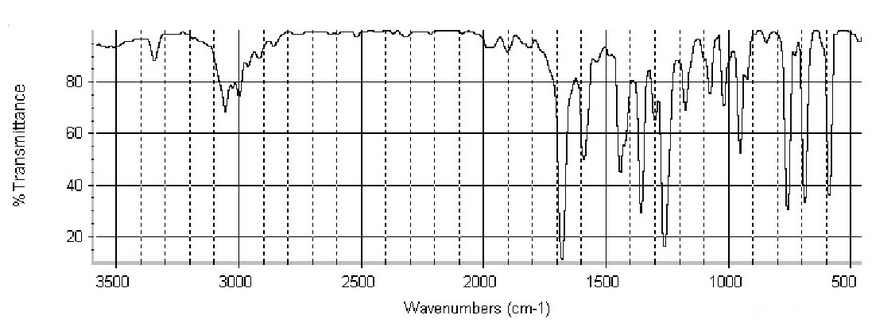
\includegraphics[scale=0.48]{images/quiz-4.png}
  \end{center}
  \medskip
  \begin{itemize}
    \item {\footnotesize\chemfig{*6(---(=O)---)}}
    \qquad {\footnotesize\chemfig{*6(-=-(-OH)-=--)}}
    \qquad {\footnotesize\chemfig{*6(-=-(-(=[:90]O)-[:-30])=-=)}}
  \end{itemize}
  \bigskip

  \basec{\begin{itemize}
    \item The large and sharp peaks at around 1700 indicate some kind of carbonyl, and there is no large broad shape indicating OH, so either first or third option.
    \item The peak around 3000--3100 indicates that some kind of C-H bond is present, specifically an \(sp^2\) hybridized carbon. 
  \end{itemize}}
  \item The two most abundant isotopes of boron are 10B and 11B, with 11B being about 4 times more abundant. In the mass spectrum of trimethylborate \ch{(CH3O)3B}.
  \begin{itemize}
    \item the peaks at m/z 103 and m/z 104 have equivalent intensities
    \item the peak at m/z 103 has an intensity which is 4 times that of the m/z 104 peak
    \item the peak at m/z 103 has an intensity which is 1/4 the intensity of the peak at m/z 104
    \item none of the above
  \end{itemize}
  \basec{\begin{itemize}
    \item \(^{11}B\) would have a peak that is one mass unit higher than \(^{10}B\), so that makes it 103 and 104 respectively.  
    \item The more abundant peak would have a higher relative intensity. 
  \end{itemize}}
  
  \item The mass spectrum of which compound has M+ and M+2 peaks of approximately equal intensity?
  \begin{itemize}
    \item 3-boromopentane
    \item 3-pentanol
    \item pentane
    \item 3-chloropentane
  \end{itemize}

  \basec{\begin{itemize}
    \item M + 2 peaks help determine any halides that are present. 
      \begin{itemize}
        \item Chlorine has 3:1 ratio due to natural occurrence of isotopes.
        \item Bromine has 1:1 ratio due to natural occurrence of isotopes.
      \end{itemize}
  \end{itemize}}
\end{enumerate}  
\clearpage
\section{Week 3/4 --- Chapter 16}\label{Week 3}
\begin{enumerate}
  \item What is the major product for the following reaction.

  \schemestart{}
    \chemfig{-[:-30](-[:-90]OH)-[:30]-[:-30]-[:30]}
    \arrow{->[\ch{CrO3}][\ch{H2SO4}]}[0,1.2]
  \schemestop{}
  \bigskip
  \begin{multicols}{2}
    \begin{itemize}
      \item \chemfig{-[:-30](=[:-90]O)-[:30]O-[:-30]-[:30]-[:-30]}
      \item \chemfig{-[:30]O-[:-30](=[:-90]O)-[:30]-[:-30]-[:30]}
      \item \chemfig{-[:-30](=[:-90]O)-[:30]-[:-30]-[:30]}
      \item \chemfig{-[:-30](-[:-90]OH)(-[:90]OH)-[:30]-[:-30]-[:30]}
    \end{itemize}
  \end{multicols}
  \basec{\begin{itemize}
    \item \ch{CrO3} is an oxidizing agent, which means electron density will be pulled away from the carbon to form a double bonded oxygen.
    \item Oxygen does not insert itself into the chain.
  \end{itemize}}
  \item Give the major product for the following oxidation.

  \medskip
  \schemestart{}
    \chemfig{(-[:90])(-[:-150])-[:-30]-[:30]-[:-30]OH}
    \arrow{->[PCC]}
  \schemestop{}
  \bigskip
  
  \begin{multicols}{2}
    \begin{itemize}
      \item \chemfig{(-[:90])(-[:-150])-[:-30]-[:30](=[:90]O)-[:-30]OH}
      \item \chemfig{(-[:90])(-[:-150])-[:-30]-[:30](=[:90]O)}
      \item \chemfig{-[:-30]-[:30]-[:-30]-[:30](=[:90]O)-[:-30]OH}
      \item \chemfig{-[:-30]-[:30]-[:-30]-[:30](=[:90]O)}
    \end{itemize}
  \end{multicols}

  \basec{\begin{itemize}
    \item PCC is a mild oxidizing agent that is commonly used for selective oxidation of alcohols to aldehydes or ketones. 
    \item In this case we started with a terminal enol, which would produce an aldehyde.
    \item The carbonyl group is not affected, it should not change.
  \end{itemize}}
  \newpage
  \item What is the major product from the following reaction?

  \medskip
  \schemestart{}
    \chemfig{-[:30]-[:-30](-[:90]Br)(-[:-90]Br)-[:30]-[:-30]}
    \arrow{->[2 \ch{NH2^{\fminus}}][]}[0,1.3]
  \schemestop{}
  \bigskip
  \begin{multicols}{2}
    \begin{itemize}
      \item \chemfig{-[:30]-[:-30](-[:-90,.8]Br)=[:30]-[:-30]}
      \item \chemfig{-[:-30]-~-}
      \item \chemfig{-[:30]-[:-30]-[:30]=[:-30]}
      \item[]
      \item \chemfig{-[:30]-[:-30]-~}
    \end{itemize}
  \end{multicols}

  \basec{\begin{itemize}
    \item This looks like dihaloalkane elimination. I took this quiz a week early, so this explanation might not be the best, but looks like \ch{NH2-} is acting as a reducing agent(?); causing the elimination of bromine, leaving the carbon to form a triple bond. 
  \end{itemize}}
  \item The major product of a hydroboration oxidation reaction on a terminal alkyne is
  \begin{multicols}{2}
    \begin{itemize}
      \item a carboxylic acid
      \item ketone
      \item alkane
      \item aldehyde
    \end{itemize}
  \end{multicols}

  \basec{\begin{itemize}
    \item Example of an alkyne undergiong a hydroboration-oxidation reaction:
      
      \medskip
      \hspace{25pt}\chemfig{\cadn{H}-[,1.2]\cadp{BH_2}}\\
      \medskip
      \schemestart{}
        \chemfig{R-\cadp{C}~\cadn{C}-H}
        \arrow{->[\ch{B2H6}][{\small\ch{H2O2}, \ch{NaOH, THF}}]}[0,1.8]
        \chemfig{(-[:150]\bbb{H})(-[:-150]R)=(-[:30]\rrr{BH_2})(-[:-30]H)}
        \arrow{->[{\small\ch{H2O2}, \ch{NaOH, THF}}]}[0,1.8]
        \dots
      \schemestop{}
      \medskip

      \medskip
      \schemestart{}
        \dots
        \quad
        \chemname{\chemfig{(-[:150]H)(-[:-150]R)=(-[:30]OH)(-[:-30]H)}}{enol}
        \arrow{<->>}
        \chemname{\chemfig{(-[:135]H)(-[:-135]R)(-[180])-(=[:30]O)(-[:-30]H)}}{aldehyde (a ketone)}
      \schemestop{}
      \bigskip
  \end{itemize}}
  \end{enumerate}
\clearpage


\section{Week 2 --- Chapter 15}\label{Week 2}
\begin{enumerate}
  \item The reagent needed to convert 2-butyne to cis-2-butene is
  \begin{itemize}
      \item \ch{H2/Pd-C}
      \item \ch{Li/NH3}
      \item \ch{Na/NH3}
      \item \ch{H2/Lindlar Catalyst}
    \end{itemize}
    \basec{\begin{itemize}
    \item Complete hydrogenation of an alkyne:
      
    \medskip
    \schemestart{}
      \chemfig{R-~-R'}
      \arrow{->[\ch{H2}][Pd-c]}
      \chemfig{R-(-[:90]H)(-[:-90]H)-(-[:90]H)(-[:-90]H)-R'}
    \schemestop{}
    \bigskip

    \item Alkyne \to\ \emph{cis}-alkene; use of lindlar catalyst (Pd-c poisoned with lead) limits further reduction by controlling hydrogens available:
    
    \medskip
    \schemestart{}
    \chemfig{R-~-R'}
    \arrow{->[\ch{H2}][lindlar]}
    \chemfig{(-[:150]H)(-[:210]R)=(-[:30]H)(-[:-30]R')}
    \schemestop{}
    \bigskip
    
    \item Alkyne \to\ \emph{trans}-alkene; using generation of free radicals (\bbb{\bullet}, single electron) that pair up with another electron generated by the dissociation of Na \to\ \rrr{\ch{Na+}}\plus\ \bbb{\ch{e-}} to create a free pair of electrons that then receive a hydrogen from \ch{NH3}:

    \medskip
    \schemestart{}
      \chemfig{R-~-R'}
      \arrow{->[Na][liq. \ch{NH3}]}
      \chemfig{(-[:120,.3,,,draw=none]\bbb{\bullet})(-[:-150]R)=(-[:30]R')(-[:-60,.3,,,draw=none]\bbb{\bullet})}
      \arrow{->}
      \chemfig{(-[:120,.3,,,draw=none]\bbb{\ani})(-[:-150]R)=(-[:30]R')(-[:-60,.3,,,draw=none]\bbb{\ani})}
      \dots
    \schemestop{}
    \bigskip

    \medskip
    \schemestart{}
      \dots
      \arrow{->[\ch{H-NH2}]}[0,1.2]
      \chemfig{(-[:150]H)(-[:210]R)=(-[:30]R')(-[:-30]H)}
    \schemestop{}
    \bigskip
  \end{itemize}}

  \item A mixture of 1-heptyne, 2-heptyne, and 3-heptyne was hydrogenated in the presence of a palladium catalyst until hydrogen uptake stopped. If one assumes that the hydrogenation went to completion for all the reactants present in the mixture, how many distinct seven-carbon isomers were produced?
  \begin{itemize}
    \item 0nly 1
    \item 2
    \item 4
    \item 6
  \end{itemize}

  \basec{
    \begin{itemize}
      \item \ch{H2/Pd-c} (palladium catalyst) generates completely saturated alkenes, thus the location of the double bond in a heptyne will make no difference overall.
    \end{itemize}}

  \item Give the best reagents for the reaction
  
  \medskip
  \schemestart{}
    \chemfig{\ch{(CH3)2CHCH2C}-[,1.7,,,draw=none]~CH}
    \arrow{}
    \chemname[-25pt]{\chemfig{\ch{(CH3)2CHCH2CH2CH}-[:-7,1.75,,,draw=none](=[:-90]OH)}}{}
  \schemestop{}
  \bigskip
  \begin{itemize}
    \item \ch{H2O}, \ch{H2OSO4}, \ch{HgSO4}
    \item \ch{BH3}, \ch{H2O2}, \ch{NaOH}
    \item \ch{K2Cr2O7}
    \item \ch{H2}, Lindlar Catalyst
  \end{itemize}
 
  \basec{\begin{itemize}
    \item First, this is a hydration reaction, so that limits just the first two options. 
    \item Hydration using \ch{H2O} and \ch{H2OSO4} or \ch{HgSO4} does have difference, but both follow Markovnikov's rule and end produce internal enols and thus internal ketones.
    \item Hydroboration-oxidation reaction follows anti-Markovnikov rule and produces a terminal enol and thus an aldehyde, which is the desired product.
  \end{itemize}}

  \item Which of the alkyne addition reactions below involves an enol intermediate?
  \begin{itemize}
    \item Hydroboration/oxidation
    \item dil. \ch{H2SO4} in \ch{HgSO4}
    \item Hydrogenation
    \item Both hydroboration/oxidation and dil. \ch{H2SO4} in \ch{HgSO4}
  \end{itemize}
  \basec{
    \begin{itemize}
      \item See question three, both hydroboration/oxidation and dil. \ch{H2SO4} in \ch{HgSO4} are used in hydration, which have enol intermediates.
      \item Hydrogenation only has to do with adding hydrogens to saturate the alkyne through elimination reactions, which question one covers. 
    \end{itemize}}
\end{enumerate}

\clearpage
\section{Week 1 --- Chapter 14}\label{Week 1}
\begin{enumerate}
    \item Name the structure: 
    
    \medskip
    \schemestart{}
        \chemfig{*7((-Cl)--=----)}
    \schemestop{}
    \bigskip
    
    \begin{itemize}
      \item 1-chloro-3-cycloheptene
      \item 4-chloro-1-cycloheptene
      \item 4-chloro-1-cyclohexene
      \item 6-chloro-1-cycloheptene
      \basec{\begin{itemize}
        \item When numbering the parent chain, the double bond should receive the lowest number possible; \emph{k=1}
          \begin{itemize}
            \item Note: define the location \(k\) of the double bond as being the number of its first carbon, not at the end.
          \end{itemize}
        \item The locant (\(k\)) of the double bond should be placed right before the suffix of ``ene,'' though, it was previously recommended before the parent (both are acceptable), e.g., 2-pentene = pent-2-ene; \emph{1-cycloheptene}
        \item Name and the side groups (other than hydrogen) according to the appropriate rules; \emph{chloro}
        \item Define the position of each side group as the number of the chain carbon it is attached to; \emph{4-}
      \end{itemize}}
    \end{itemize}

    \item Name the structure: 
    
    \medskip
    \schemestart{}
      \chemfig{ClCH_2CH_2-[:-30](-[:210]H)=(-[:-30]H)
      (-[:30]C(-[:150]H)=(-[:-30]H)-[:30]CH_3)
      }
    \schemestop{}
    \bigskip

    \begin{itemize}
      \item (2E,4E)-7-chloro-2,4-heptadiene
      \item (2Z,4Z)-7-chloro-2,4-heptadiene
      \item (2Z,4E)-7-chloro-2,4-heptadiene
      \item (2E,4Z)-7-chloro-2,4-heptadiene
      \basec{
        \begin{itemize}
          \item \ddd{E-Z notation}: recommended instead of \textit{cis} and \textit{trans} in order to account for cases that has more than two different groups attached to the double bond by first determining the priority using the \link{https://en.wikipedia.org/wiki/Cahn\%E2\%80\%93Ingold\%E2\%80\%93Prelog_priority_rules}{Cahn-Ingold-Prelog System}.
          \begin{itemize}
            \item \fff{E, entgegen, ``opposite''}.
            \item \ttt{Z, zusammen, ``together''}; ``on ze zame zide.''
        \end{itemize}
        \item When numbering the parent chain, the double bond should receive the lowest number possible; \emph{k=2}
          \begin{itemize}
            \item The two highest priority groups are on \fff{opposite} sides; \emph{2E}
          \end{itemize}
        \item There is more than one double bond; \emph{\(k_2=4\)}
          \begin{itemize}
            \item The two highest priority groups are on \ttt{zame} side; \emph{4Z}
          \end{itemize}
      \end{itemize}
      }
    \end{itemize}
    
    \item How many stereoisomeric product(s) do you get in the reaction below.
    
    \medskip
    \schemestart{}
      \chemfig{=[:30]-[:-30](-[:30]-[:-30])-[:-90]-[:-30]}
      \arrow{->[\ch{Hg(OAc)2}, \ch{H2O}, THF][\ch{NaBH4}]}[0,2.2]
    \schemestop{}
    \bigskip
    
    \basec{\begin{itemize}
      \item Oxymercuration-demercuration reactions follow Markovnikov's rule, i.e., \rrr{\(H^+\)} is added to the carbon with the \rrr{greatest} number of hydrogen atoms while the \bbb{\(X^-\) component} is added to the carbon with the \bbb{fewest} hydrogen atoms.
      \item Drawing the intermediate is not necessary, and no chiral centers are found in the products:
      
      \medskip
      \schemestart{}
        \dots 
        \arrow(--[braces]){->[\rrr{\ch{Hg(OAc)2}}, \bbb{\ch{H2O}}, THF][\ch{NaBH4}]}[0,2.2]
        \chemfig{\rrr{H}-[:30](<[:90]\bbb{OH})-[:-30](-[:30]-[:-30])-[:-90]-[:-30]}
        \+
        \chemfig{\rrr{H}-[:30](<:[:90]\bbb{OH})-[:-30](-[:30]-[:-30])-[:-90]-[:-30]}
      \schemestop{}
      \bigskip
      
    \end{itemize}}
    
    \item Which reaction intermediate is formed when Br2/CCl4 reacts with cyclohexene?
    
    \begin{multicols}{2}
    \begin{enumerate}[label=\roman*]
    
    \item 

    \medskip
    \schemestart{}
      \chemfig{*6(--(-[,.3,,,,draw=none]\cat)-(-Br)---)}
    \schemestop{}
    \bigskip

    \item 

    \medskip
    \schemestart{}
      \chemfig{*6(--(-Br)-(-[,.3,,,,draw=none]\cat)---)}
    \schemestop{}
    \bigskip

    \item 

    \medskip
    \schemestart{}
      \chemfig{*6(--(-[,.3,,,,draw=none]\cdot)-(-Br)---)}
    \schemestop{}
    \bigskip

    \item 

    \medskip
    \schemestart{}
      \chemfig{*6(--(-[:30]Br\,\cat)-(-[:-30,.55])---)}
    \schemestop{}
    \bigskip

    \item 

    \medskip
    \schemestart{}
      \chemfig{*6(--(-Br)-(-Br)---)}
    \schemestop{}
    \bigskip

    \end{enumerate}
    \end{multicols}

    \basec{\begin{itemize}
      \item \ddd{Halogenation}: a reaction that involves the addition of one or more halogens to a compound or material.
    \begin{itemize}
      \item The addition of halogens to alkenes proceeds via \emph{intermediate halonium ions}.
      \item \ddd{Halonium ion}: any onium ion containing a halogen atom carrying a positive charge. This cation has the general structure: \chemfig{R-[,.7]\rrr{+X}-[,.7]R'}
      \item \ddd{Onium ion}: a \rrr{cation} formally obtained by the protonation of mononuclear parent hydride of a pnictogen (group 15 of the periodic table), chalcogen (group 16), or halogen (group 17); \rrr{\(Br^\cat \)} in our case.
    \end{itemize}
    \end{itemize}}
\end{enumerate}
\end{document}